
%Ultimate Formal Report Template 		Author: Dylan Morano ©
%
%Feel free to edit and redistribute 
%
%-------------------------------Document Information-------------------------------%

\newcommand{\Report}		{OCE-408 Final Project}			%Report Name
\newcommand{\Author}		{Dylan Morano, Rebecca Cressman, Arielle De Souza, Scott Hara}		%Author
\newcommand{\Last}		{Morano, Cressman, De Souza, Hara}				%Authors Last Name
\newcommand{\Class}		{OCE-311}			%Class Title
\newcommand{\Professor}	{Jason Dahl}			%Professor(s)

%----------------------------------------Preamble---------------------------------------%

\documentclass[10pt,letterpaper,titlepage]{report}
\usepackage[toc,page]{appendix}	%appendix support
\usepackage{fixltx2e}	%official latex patch and fixes
%\usepackage[latin1]{inputenc} 	%accepts different input encodings
\usepackage{pdflscape}	%landscape support
\usepackage{multicol}	%multicolumn support
\usepackage{setspace}	%set line spaceing (double single half)
\usepackage{geometry}	%change page geometry (margins)
\usepackage{datetime}	%automatic date/time insertion
\usepackage{fancyhdr}	%fancy headers
\usepackage{titlesec}	%Select alternative section titles
\usepackage{hyperref}	%support hypertext referencing
\usepackage{paralist} 	%enumerate and itemize within paragraphs
\usepackage{tabu}		%flexible latex tabulars
\usepackage{amsmath}	%facilitates math formulas and equations
\usepackage{amsfonts}	%math fonts and symbols
\usepackage{amssymb}	%more symbols
\usepackage{graphicx}	%enhanced support for graphics
\usepackage{subfigure}	%multiple figure containment
\usepackage{caption}	%figure captions
\usepackage{float}		%float figures within text
\usepackage{epstopdf}	%.EPS file support
% \usepackage{subfig}		%subfigures
% \usepackage{subcaption}	%subcaptions
\usepackage{listings}	%code and listing input
\usepackage{mcode} 	%MATLAB code parsing mcode.sty required in working directory
\usepackage{color} 		%custom color packaging
\usepackage{apacite}	%citing APA format

%	Define margins
\geometry{top = 1.0in, bottom = 1.0in, left = 1.0in, right = 1.0in}

%	Double spacing
\doublespacing

%	\Hide command for hiding section tidles
\newcommand*\Hide{
\titleformat{\chapter}[display]
  {}{}{0pt}{\bf \Huge}
\titleformat{\part}
  {}{}{0pt}{}
}

%	Define colors for matlab insertion
\definecolor{mygreen}{RGB}{28,172,0}  
\definecolor{mylilas}{RGB}{170,55,241}

%	define default path to graphic files
\graphicspath{ ../figures}


%	Declare types of images
\DeclareGraphicsExtensions{.pdf,.png,.jpg,.eps}


%------------------------------------------------------Begin Document------------------------------------------------------%

\begin{document}

\title{\Report}
\date{\today}
\author{\Author \\ \Class \\ \Professor}	

\pagenumbering{arabic}
\rhead{\Last}
\lhead{\Report}
\pagestyle{fancy}

%	print titlepage
\maketitle

%	print Abstract
% \section*{Abstract}
% \newpage

%	print table of contents
\tableofcontents

%	print lists of content
\listoffigures
%\listoftables
%\listofequations

%--------------------------------Begin Sections--------------------------------%
\newpage
\Hide
\chapter{Introduction}

Narragansett Town Beach is an important economic resource to the town of Narragansett, providing an average net income of $\$$270,000 each season and increasing seasonal business for surrounding restaurants, shops, and rentals. It is important to understand the natural forces which contribute to beach erosion for expensive re-nourishment project in order to keep the beach healthy for vacationers. In order to understand these processes, a study was conducted utilizing data from the Wave Informations Studies (WIS) program. 20, and 50 year return storm waves projected towards the beach were analyzed in order to determine incident wave rays and breaking characteristics. This information can then be used in order to determine the littoral processes present at Narragansett Beach. 
\chapter{Task 1}

\section{Statement of Problem}

\section{Hypotheses and Theories}



\section{Solution of the Problem}

\section{Conclusion}

\newpage
\Hide
\chapter{Task 2}

\section{Statement of Problem}
Task 2 utilizes a wave ray tracing algorithm and local bathymetry information, provided for Narragansett Bay, in order to propagate storm waves determined from task 1. In order to complete this task, simulations are conducted for the 20 and 50 year storms along with creating rays that intersect along the shoreline of Narragansett Beach. For the 20 year storm simulations, use the ray spacing on the beach to calculate a refraction coefficient for each section of beach. Then, using bathymetry data from a chart near the beach, estimate the beach slope. This is used along with the deep water wave properties and refraction coefficient to estimate the shoaling coefficient, breaking depth, and breaker height. 
\section{Hypotheses and Theories}

When waves propagate over a non uniform sea floor, they refract depending on how the sea floor depth changes along the wavefront. As water depth decreases wave fronts can focus or de-focus along the coastline. Seen in \ref{eq:refrac_coeff}, the refraction coefficient can be determined with the distance between wave rays initially, and in the target location. A refraction coefficient less than one indicates de-focusing. 

\begin{equation}
K_{r} = \sqrt{\dfrac{b_{o}}{b}}
\label{eq:refrac_coeff}
\end{equation}

In shallow water, waves slow down and experience an increase in wave height due to shoaling. The degree of wave refraction, and the shoaling coefficient dictate breaking wave height and water depth. Seen in \ref{eq:shoaling_coeff}, the ratio of phase speed and group celerity changes as water depth approaches the shallow water condition. With the deep water characteristics, and angle of incidence, breaker depth and wave height can be found iteratively.

\begin{align}[H]
c = c_{o} * \tanh(kh); \\
c_{g} = \dfrac{c}{2} * \left(1 + \dfrac{2kh}{\sinh(2kh)}\right) \\
K_{s} = \sqrt{c/2c_{g}}
\label{eq:shoaling_coeff}
\end{align}

\begin{align}
H_{b} = H_{o}K_{sb}K_{rb} = \kappa h_{b}
\\ K_{sb} = F(L,h)
\\K_{rb} = F(L,h,\theta_{o})
\label{eq:breaker_char}
\end{align}

The programs supplied for the problem simulated waves propagating into the region of coastline surrounding Narragansett Beach. The programs required deep water wave characteristics, and latitude-longitude grid resolution. 

\section{Solution of the Problem}

Using the supplied C functions and waveray.m, wave rays were simulated propagating into Narragansett Beach under the conditions determined in Task 1. Twenty and fifty year predicted wave parameters were used to simulate the path lines extreme waves followed. Seen in Figure 1.2, three predominant angles of incidence were determined from the supplied data. Waveray.m didn't allow for significant manipulation of the rendered area without ruining the data. None of the simulations intersected the coastline with more than two or three renders.

Seen below, the wave rays in all three simulations indicated that wavefronts de-focus slightly as they propagate into the bay. Figure \ref{fig:20y150deg} displayed a low degree of focusing or de-focusing along the shoreline. Waves propagating at that angle of incidence didn't experience a large reduction in wave energy before they hit the beach. Figures \ref{fig:20y180deg} and \ref{fig:20y210deg} displayed significant de-focusing as they approached the coastline. Waves that impacted the beach from those angles of incidence did so at a lower energy. The 50 year wave ray simulations can be observed in the Appendix. The simulated rays displayed identical wave propagation patterns at each angle of incidence when compared to the 20 year simulations.

\begin{figure}[H]
\centering
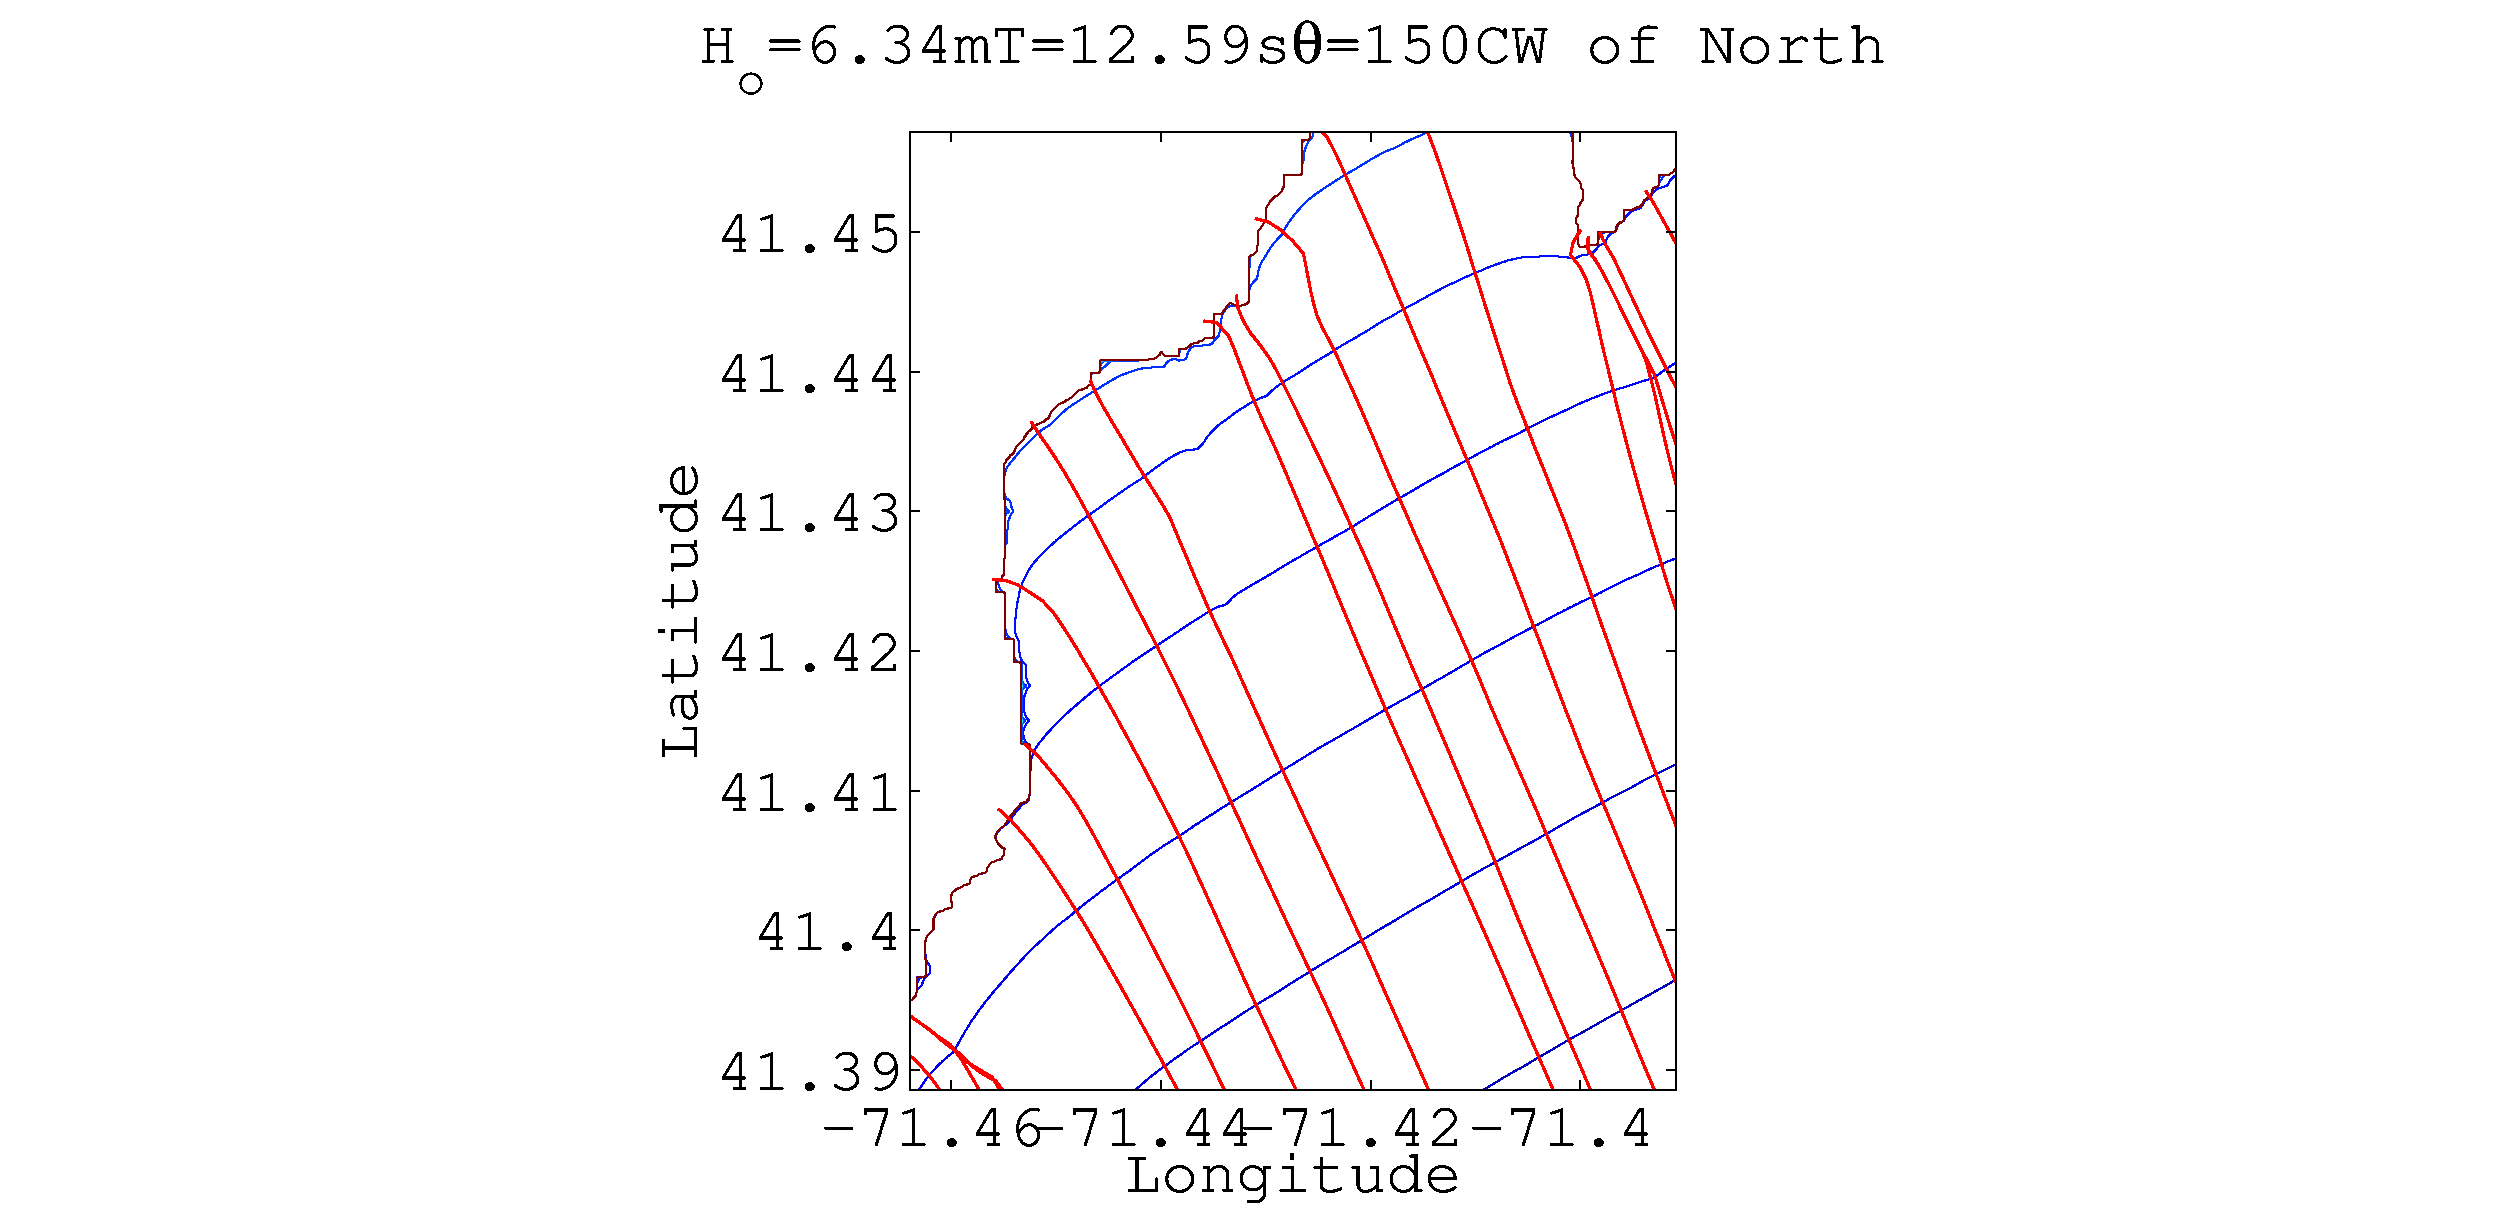
\includegraphics[width=1.0\textwidth]{./img/20y_150deg.pdf}
\caption{20y Predicted Wave Rays at 150$^{\circ}$ angle of incidence}
\label{fig:20y150deg}
\end{figure}


\begin{figure}[H]
\centering
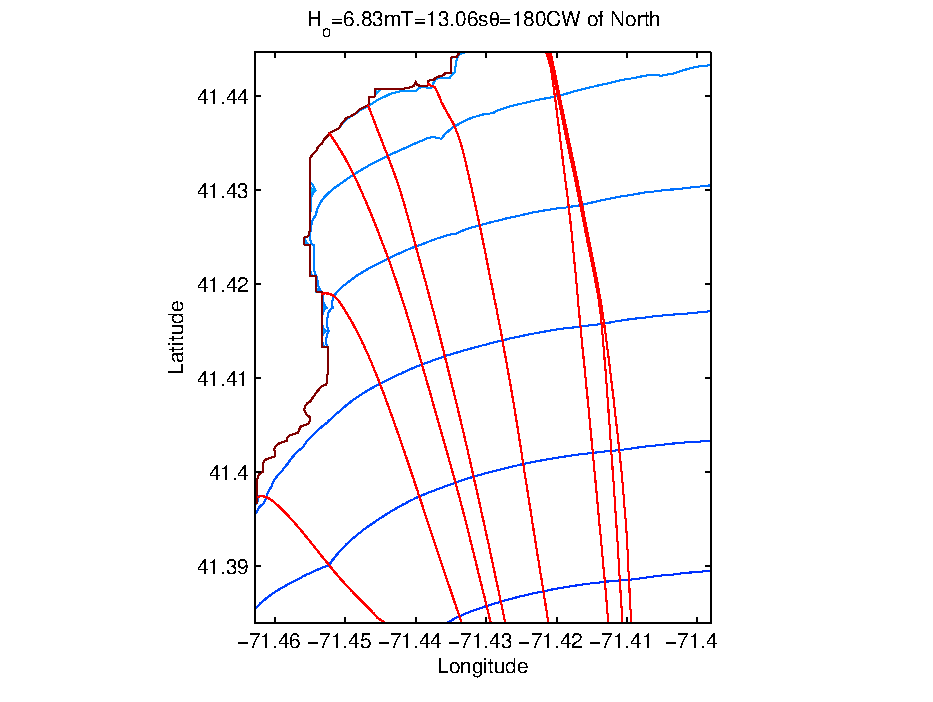
\includegraphics[width=0.6\textwidth]{./img/20y_180deg.pdf}
\caption{20y Predicted Wave Rays at 180$^{\circ}$ angle of incidence}
\label{fig:20y180deg}
\end{figure}

\begin{figure}[H]
\centering
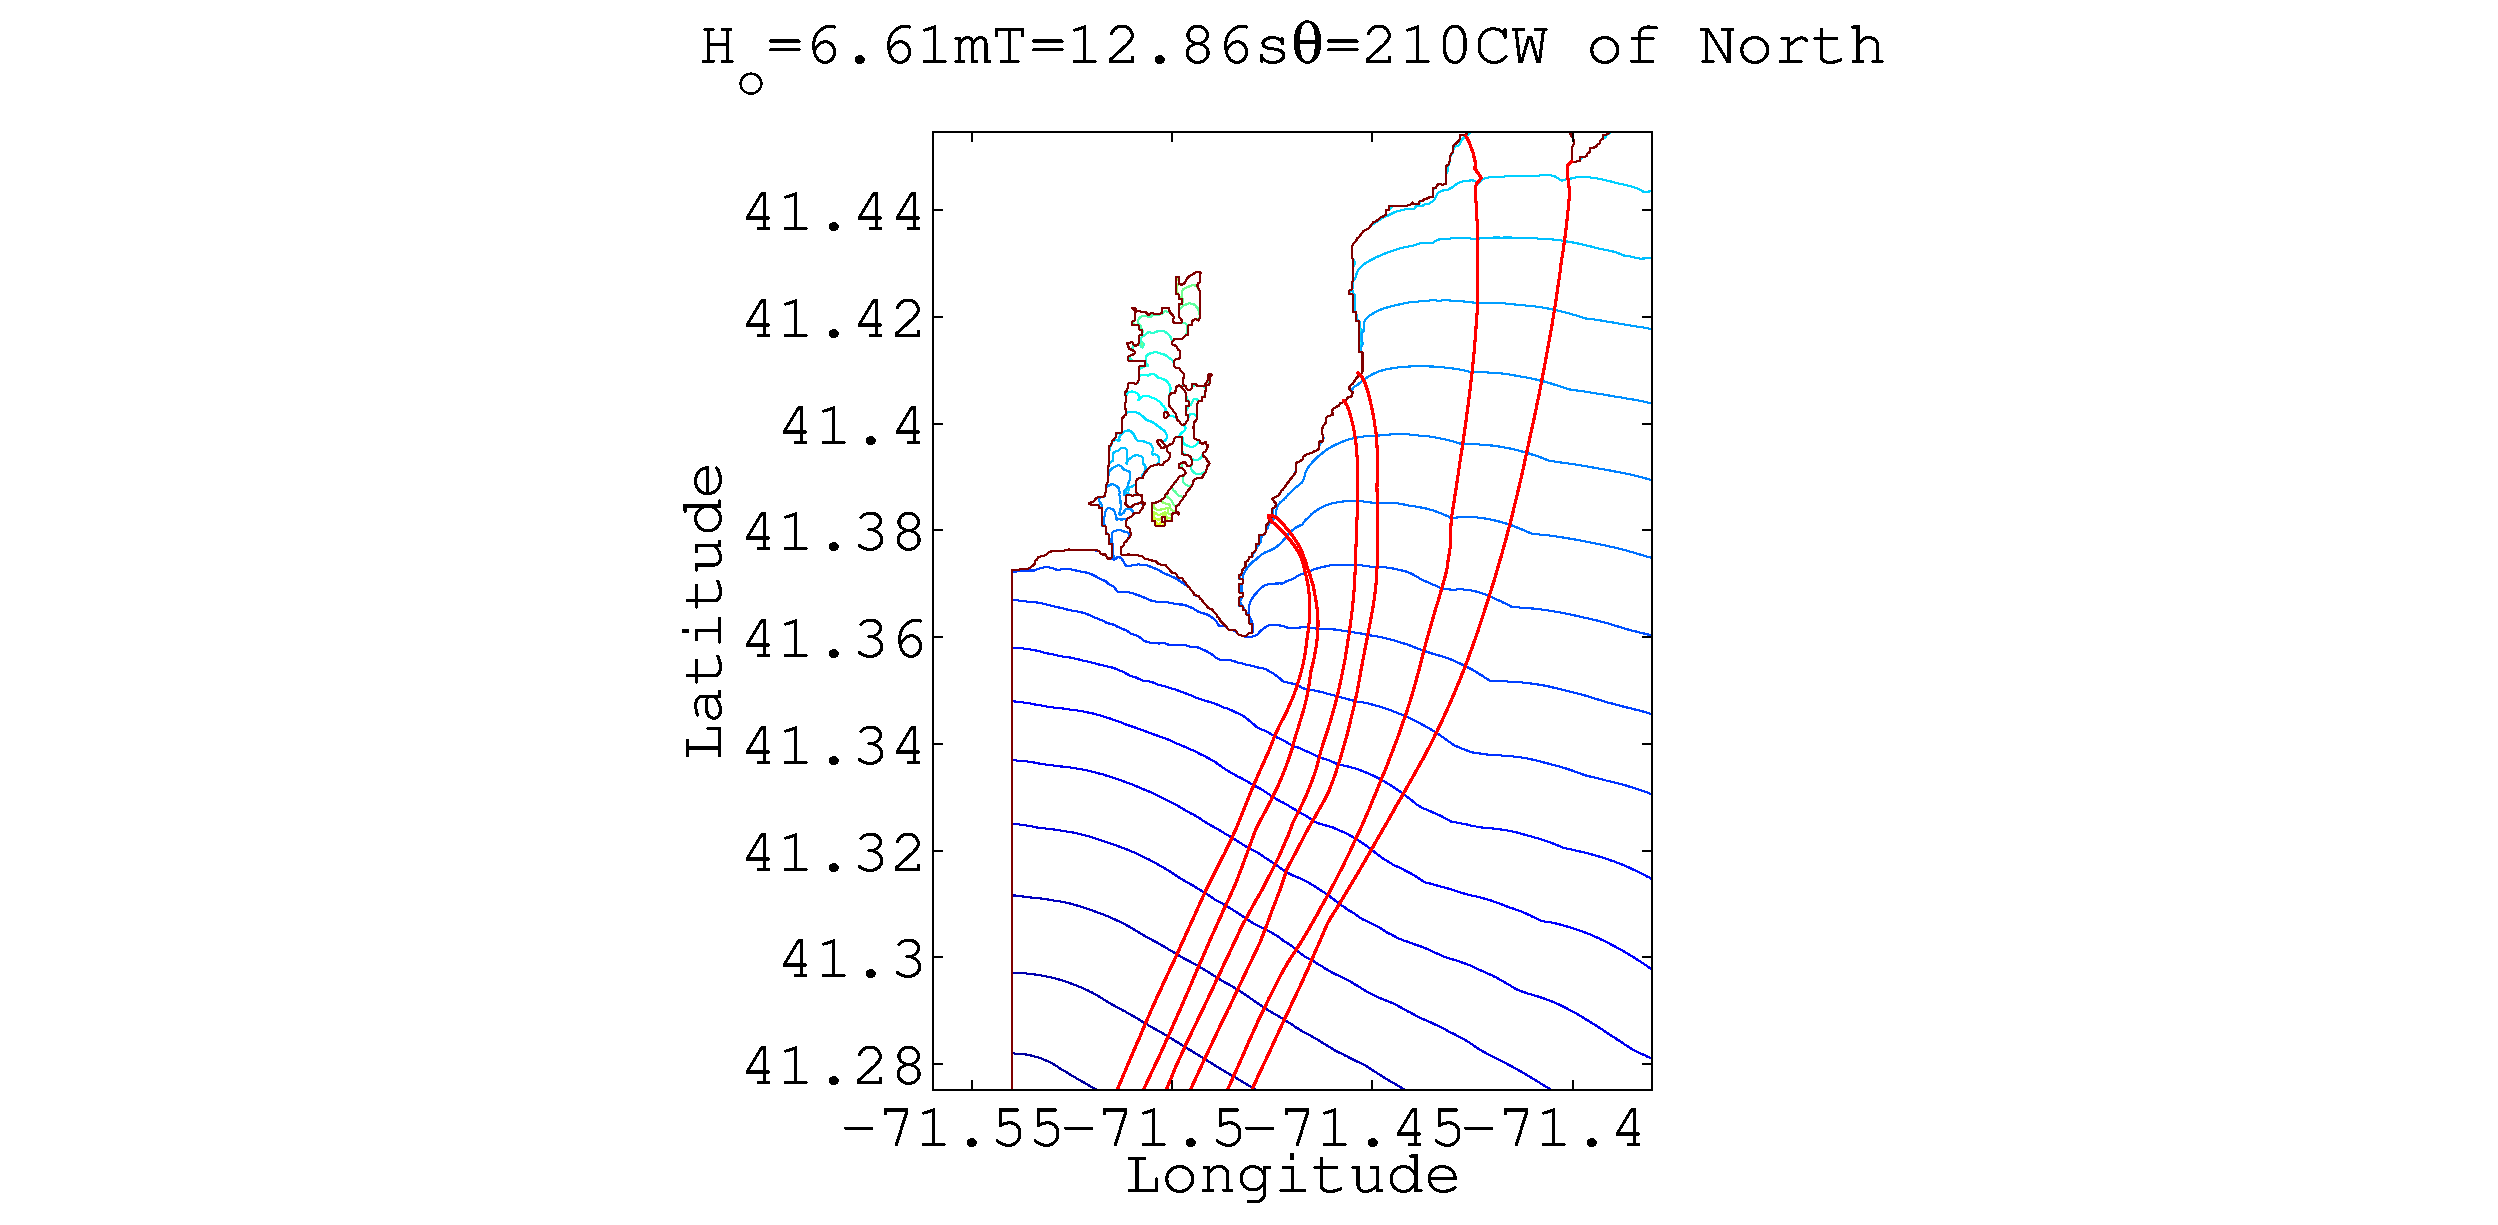
\includegraphics[width=1.0\textwidth]{./img/20y_210deg.pdf}
\caption{Breaking Wave Characteristics for 20 Year extreme wave at 210$^{\circ}$ angle of incidence}
\label{fig:20y210deg}
\end{figure}

Seen below, breaking wave characteristics were estimated using the simulated wave rays. The low number of data points impacted the breaking wave analysis by reducing its accuracy significantly. No calculations were possible for the 20 and 50 year wave ray simulations at a 210$^{\circ}$ because they did not have any rays intersecting the beach. The values that could be calculated for the remaining simulations were incorrect. Tables \ref{tab:20y_150deg} and \ref{tab:50y_150deg} indicated that the breaking wave characteristics were scaling properly with more extreme initial wave conditions.

\begin{table}[H]
\centering
\begin{tabular}{ccccc}
$K_{r}$ & $K_{s}$ & $H_{b}$ & $h_{b}$ & $\dfrac{H_{b}}{h_{b}}$ \\
\hline
0.0 & 0.1 & 5.2 & 7.6 & 0.7 \\
1.0 & 0.0 & 3.4 & 7.5 & 0.5 \\
\hline
\end{tabular}

\caption{Breaking Wave Characteristics for 20 Year extreme wave at 150$^{\circ}$ angle of incidence}
\label{tab:20y_150deg}
\end{table}

\begin{table}[H]
\centering
\begin{tabular}{cccccc}
Ray: & $K_{r}$ & $K_{s}$ & $H_{b}$ & $h_{b}$ & $\dfrac{H_{b}}{h_{b}}$ \\
\hline
1 & 1.0 & 0.1 & 5.8 & 8.2 & 0.7 \\
2 & 1.0 & 0.1 & 4.9 & 8.2 & 0.6 \\
\hline
\end{tabular}

\caption{Breaking Wave Characteristics for 20 Year extreme wave at 180$^{\circ}$ angle of incidence}
\label{tab:20y_180deg}
\end{table}

\begin{table}[H]
\centering
\begin{tabular}{cccccc}
Ray: & $K_{r}$ & $K_{s}$ & $H_{b}$ & $h_{b}$ & $\dfrac{H_{b}}{h_{b}}$ \\
\hline
1 & 1.0 & 0.1 & 6.2 & 8.6 & 0.7 \\
2 & 1.0 & 0.0 & 4.0 & 8.5 & 0.5 \\
\hline
\end{tabular}

\caption{Breaking Wave Characteristics for 50 Year extreme wave at 150$^{\circ}$ angle of incidence}
\label{tab:50y_150deg}
\end{table}

\begin{table}[H]
\centering
\begin{tabular}{cccccc}
Ray: & $K_{r}$ & $K_{s}$ & $H_{b}$ & $h_{b}$ & $\dfrac{H_{b}}{h_{b}}$ \\
\hline
1 & 1.0 & 0.1 & 6.8 & 9.2 & 0.7 \\
2 & 1.0 & 0.0 & 4.2 & 9.0 & 0.5 \\
\hline
\end{tabular}

\caption{Breaking Wave Characteristics for 50 Year extreme wave at 180$^{\circ}$ angle of incidence}
\label{tab:50y_180deg}
\end{table}


%Talkin bout sediment transport
Sediment transport 

%Talkin bout wave energy facility and location importance and such
Placement of a wave energy facility within Narragansett Bay can be determined with the help of the data analysis used for this project. Just as it was used here, hind casting can determine yearly wave characteristics, and major angles of incidence. Wave ray simulations can identify regions of wave focusing within the bay. However, the data used in this project would not be suitable for use in evaluating average conditions of the bay. The supplied 20 and 50 year predictions were based off of the extreme conditions from each sample range. An energy spectra of waves in the region would be required instead of a Gumbel distribution. Average wave parameters can be found using the energy spectra, providing more reasonable characteristics for simulation.


%Talkin bout inclusion of diffraction model
Diffraction modeling would have influenced our 210$^{\circ}$ angle of incidence waves. Bloc

\section{Conclusion}
After manually evaluating the breaking wave characteristics, it indicated that the simulated wave rays would experience de-focusing. From the data in task 1, the simulated wave rays for the 50 year extreme showed similarity to their 20 year counterparts. Narragansett Beach also de-focused the rays that hit the beach. The degree of de-focusing can be observed to increase as the angle of incidence approaches 210$^{\circ}$ . Overall, using the supplied functions given, the wave ray analysis on Narragansett Beach under the conditions determined in task 1 proved that the simulated wave rays experienced de-focusing. 



%Question 3
%In terms of the specific wave directions determined from task 1, the inclusion of diffraction models would alter the direction of the wave rays in the ray tracing analysis.Wave diffraction involves a change in direction of waves as they pass through an opening or around a barrier in their path. The amount of diffraction (the sharpness of the bending) increases with increasing wavelength and decreases with decreasing wavelength. As waves propagate in the wave directions determined from task 1, the wave from one direction might travel a different distance than the wave from another direction. When the difference in distance is a significant difference, the waves from each direction might be in a different phase. Therefore the waves would look more realistic and accurate.



%--------------------------------Begin References--------------------------------%

%	BibTex Creator: truben.no/latex/bibtex 

\newpage
\nocite{*}
\def\bibindent{1em}
\begin{thebibliography}{1\kern\bibindent}
\makeatletter
\let\old@biblabel\@biblabel
\def\@biblabel#1{\old@biblabel{#1}\kern\bibindent}
\let\old@bibitem\bibitem
\def\bibitem#1{\old@bibitem{#1}\leavevmode\kern-\bibindent}
\makeatother

\bibitem{CEM}
US Army Corps of Engineers (2002). 
$\emph{Coastal Engineering Manual}$

\bibitem{WIS}
US Army Corps of Engineers (2002). 
$\emph{Wave Information Studies Program}$ \\
\url{http://wis.usace.army.mil/}

\bibitem{WIS}
NOAA (2014). 
$\emph{Narragansett bay including newport harbor chart: 13223.}$ \\
\url{http://www.charts.noaa.gov/OnLineViewer/13223.shtml}

\end{thebibliography}

%--------------------------------Begin Appendix--------------------------------%

\begin{appendices}

\chapter{MATLAB Calculations}

%	Matlab code parser block
%-----------------------------------------------------------------
% Must have before any Matlab code

\lstset{language=Matlab, %basicstyle=\color{red},
    breaklines=true, caption={},%
    morekeywords={matlab2tikz},
    basicstyle=\tiny,
    numberstyle=\tiny,
    keywordstyle=\color{blue},%
    morekeywords=[2]{1}, keywordstyle=[2]{\color{black}},
    identifierstyle=\color{black},%
    stringstyle=\color{mylilas},
    commentstyle=\color{mygreen},%
    showstringspaces=false,%without this there will be a symbol in the places where there is a space
    numbers=left,%
    numberstyle={\tiny \color{black}},% size of the numbers
    numbersep=9pt, % this defines how far the numbers are from the text
    emph=[1]{for,end,break},emphstyle=[1]\color{red}, %some words to emphasise
    emph=[2]{word1,word2}, emphstyle=[2]{style},
    captionpos=b,					% sets the caption-position to bottom
}
%-----------------------------------------------------------------
\section{Parser Function}
\lstinputlisting{../"Task 1"/matlab/parser.m}
\section{Task 1 Script}
\lstinputlisting{../"Task 1"/matlab/task1code.m}
\section{Task 2 Waveray Script}
\lstinputlisting{../"Task 2"/matlab/"raytracing"/task2_waveray.m}
\section{Task 2 Breaker Script}
\lstinputlisting{../"Task 2"/matlab/"Breaker Line Analysis"/LATLONDIST.m}

\chapter{Task 1 Appendicies}

\section{Monthly Maximum output example}
\lstinputlisting[caption = Example output from monethextrema\_new.m, label = lst:example150, firstline = 1, lastline = 5] {../"Task 1"/matlab/monthlyExtreme63079_150.txt}

\section{Yearly Average Wave Conditions}

\begin{minipage}{0.36\textwidth}
\begin{table}[H]
	\begin{tabular}{ccc}
Year & Avg Hs(m) & Avg Ts (m)\\ \hline
1980.0 & 0.8 & 6.5 \\
1981.0 & 0.8 & 6.5 \\
1982.0 & 0.6 & 6.3 \\
1983.0 & 0.9 & 6.5 \\
1984.0 & 0.9 & 6.7 \\
1985.0 & 0.7 & 6.5 \\
1986.0 & 0.9 & 6.4 \\
1987.0 & 0.9 & 6.3 \\
1988.0 & 0.8 & 6.1 \\
1989.0 & 0.8 & 6.4 \\
1990.0 & 0.9 & 7.0 \\
1991.0 & 0.9 & 6.5 \\
1992.0 & 0.9 & 7.0 \\
1993.0 & 0.8 & 6.7 \\
1994.0 & 0.9 & 6.7 \\
1995.0 & 1.0 & 8.6 \\
1996.0 & 1.2 & 7.3 \\
1997.0 & 0.9 & 6.9 \\
1998.0 & 1.0 & 7.4 \\
1999.0 & 0.9 & 6.9 \\
\hline
\end{tabular}

	\label{yearly150}
	\caption{150$^\circ$ Yearly Averages}
\end{table}
\end{minipage}
\begin{minipage}{0.36\textwidth}
\begin{table}[H]
	\begin{tabular}{ccc}
Year & Avg Hs(m) & Avg Ts (m)\\ \hline
1980.0 & 1.0 & 6.4 \\
1981.0 & 1.0 & 6.6 \\
1982.0 & 1.0 & 6.1 \\
1983.0 & 1.0 & 6.3 \\
1984.0 & 1.1 & 6.6 \\
1985.0 & 0.9 & 6.2 \\
1986.0 & 0.9 & 6.2 \\
1987.0 & 0.9 & 6.1 \\
1988.0 & 0.9 & 6.4 \\
1989.0 & 1.1 & 6.5 \\
1990.0 & 1.0 & 6.8 \\
1991.0 & 1.0 & 6.4 \\
1992.0 & 0.9 & 6.5 \\
1993.0 & 1.0 & 6.5 \\
1994.0 & 1.1 & 6.6 \\
1995.0 & 1.1 & 7.3 \\
1996.0 & 1.1 & 7.2 \\
1997.0 & 1.0 & 7.0 \\
1998.0 & 1.0 & 7.2 \\
1999.0 & 1.0 & 6.8 \\
\hline
\end{tabular}

	\label{yearly180}
	\caption{180$^\circ$ Yearly Averages}
\end{table}
\end{minipage}
\begin{minipage}{0.36\textwidth}
\begin{table}[H]
	\begin{tabular}{ccc}
Year & Avg Hs(m) & Avg Ts (m)\\ \hline
1980.0 & 1.1 & 6.4 \\
1981.0 & 1.1 & 6.5 \\
1982.0 & 1.1 & 6.1 \\
1983.0 & 1.0 & 6.0 \\
1984.0 & 0.9 & 5.9 \\
1985.0 & 1.0 & 6.3 \\
1986.0 & 1.0 & 6.3 \\
1987.0 & 0.9 & 6.1 \\
1988.0 & 1.2 & 6.3 \\
1989.0 & 1.1 & 6.4 \\
1990.0 & 1.2 & 6.4 \\
1991.0 & 0.9 & 5.8 \\
1992.0 & 1.0 & 6.1 \\
1993.0 & 1.1 & 6.2 \\
1994.0 & 1.0 & 6.2 \\
1995.0 & 1.1 & 6.3 \\
1996.0 & 1.1 & 6.7 \\
1997.0 & 1.1 & 6.2 \\
1998.0 & 1.0 & 6.2 \\
1999.0 & 1.1 & 6.3 \\
\hline
\end{tabular}

	\label{yearly210}
	\caption{210$^\circ$ Yearly Averages}
\end{table}
\end{minipage}

\end{appendices}
\end{document}